\documentclass{article}
\usepackage[utf8]{inputenc}
\usepackage[english,russian]{babel}
\usepackage{hyperref}
\usepackage{graphicx}
\usepackage[scale=0.75]{geometry}
\usepackage{mathtools}

\title{Лабораторная работа #1}
\author{Крухмалев Константин,Рашо Елизавета,Фролова Дарья, М34371}

\begin{document}


\maketitle


\href{https://github.com/Konstantin343/optimization-methods-itmo/tree/main/lab2}{https://github.com/Konstantin343/optimization-methods-itmo/tree/main/lab2}

\section{Стохастический градиентный спуск}

\subsection{Описание}
Оптимизационный алгоритм, отличающийся от обычного градиентного спуска тем, что градиент оптимизируемой функции считается на каждом шаге не как сумма градиентов от каждого элемента выборки, а как градиент от одного, случайно выбранного элемента. \\
Выбрана функция ошибки MSE, количество используемых объектов - batch\_size, передается алгоритмы как аргумнт.  \\
Для графиков сгенерирован датасет с однмерной линейной регрессией. \\

\subsection{1 - SGD}
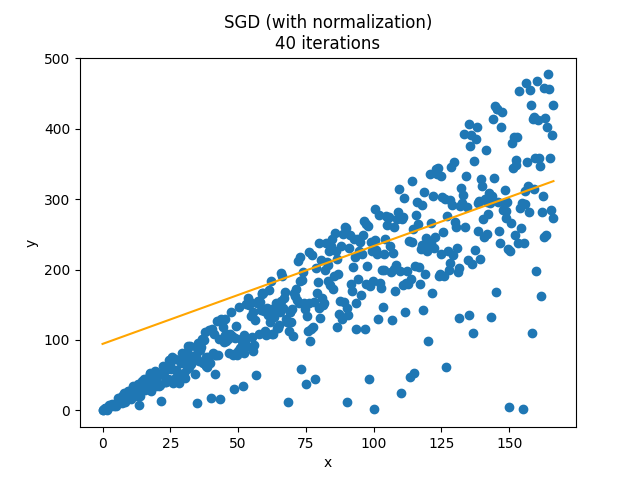
\includegraphics[scale=0.4]{sgd_points_norm.png}
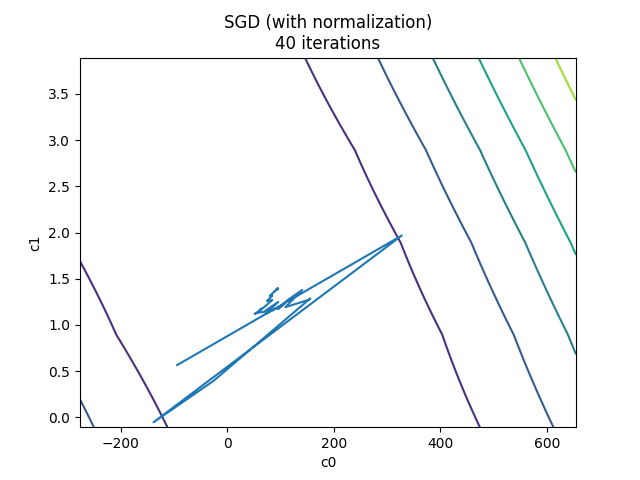
\includegraphics[scale=0.4]{sgd_trace_norm.png}

\subsection{2..n-1 - Minibatch GD}
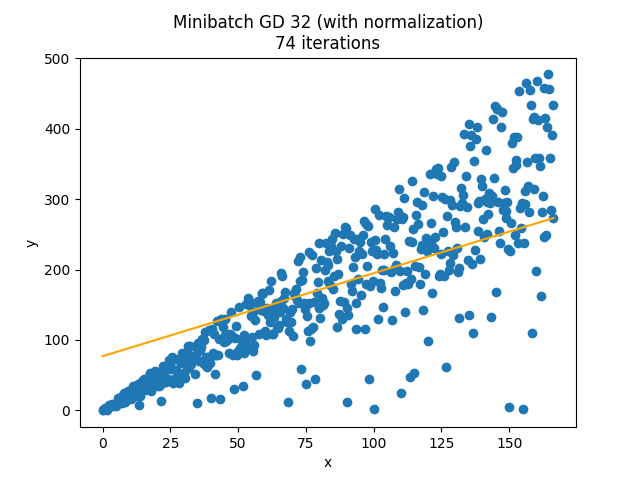
\includegraphics[scale=0.4]{minibatch_points_norm.png}
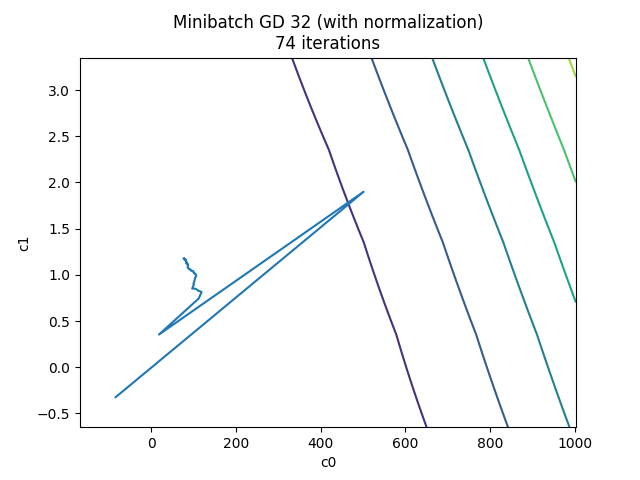
\includegraphics[scale=0.4]{minibatch_trace_norm.png}

\subsection{n - GD}
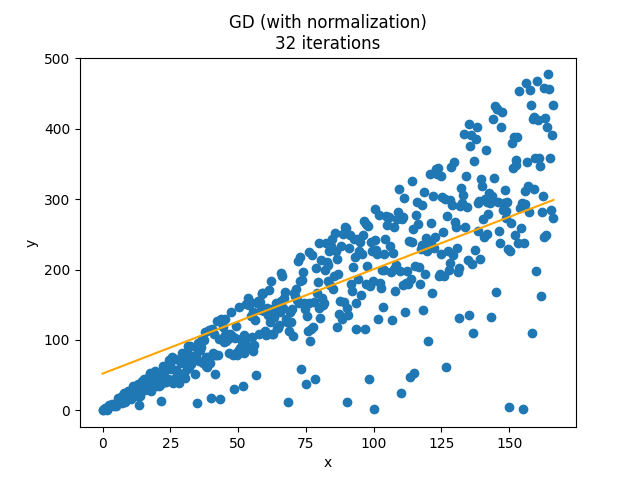
\includegraphics[scale=0.4]{gd_points_norm.png}
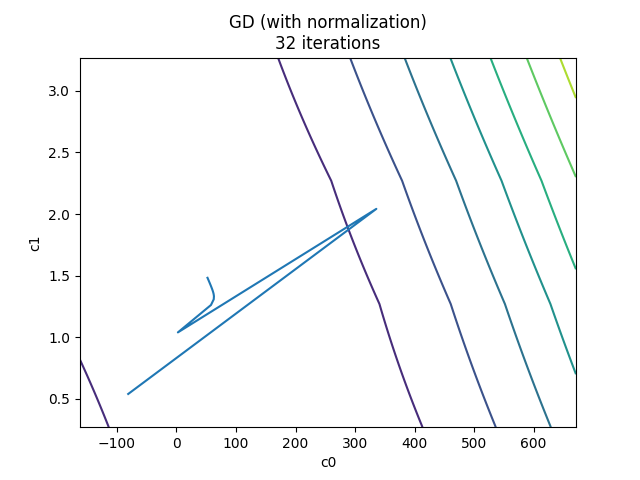
\includegraphics[scale=0.4]{gd_trace_norm.png}

\subsection{Выводы}
Наиболее точные результаты с меньшим числом итераций получены в процессе полного градиентного спуска. \\
Стохастический градиентный спуск дает наимение точные результаты, однако затрачивает меньше итераций, чем Minibatch GD и работает быстрее по времени. \\

\section{Scaling (нормализация)}

\subsection{Описание}
В лабораторной выполняетс minimax нормализация данных.\\
При нормализации для каждой координаты выполняется следующее:
$$v^{norm}_i = (v_i - min_i) / (max_i - min_i)$$
При денормализации коэффициентов выполняется следующее:
$$v_0 = min_y + \sum_{i = 1}^{n}{(v_i * min_i) / (max_i - min_i)}$$
$$v_i = v^{norm}_i / (max_i - min_i) * (max_y - min_y)$$

\subsection{Выводы}
Без предварительной нормализации во всех предыдущих примерах достигаются слишком большие значения ошибки, в следствие чего алгоритм не завершает свою работу. \\
При денормализации коэффициентов может быть потеряна точность, но алгоритм всегда завершается.

\section{Модификации градиентного спуска}

\subsection{SGD}

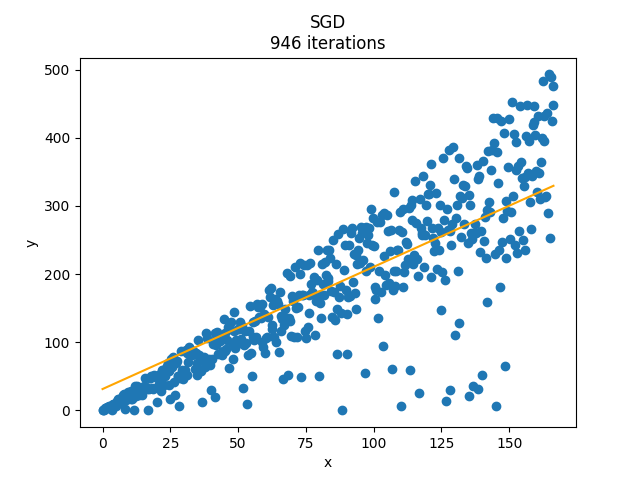
\includegraphics[scale=0.4]{sgd_points.png}
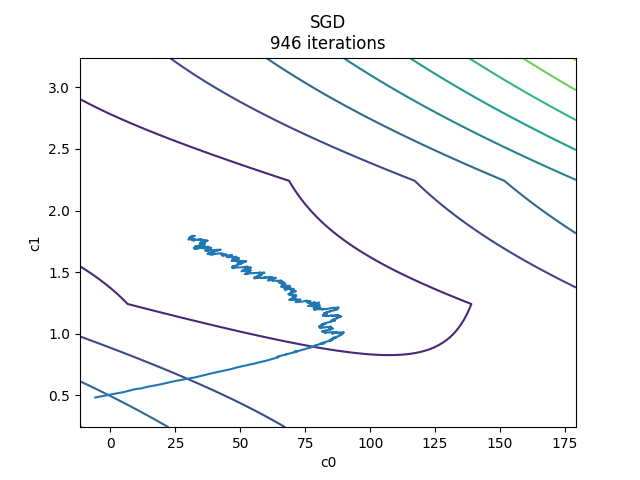
\includegraphics[scale=0.4]{sgd_trace.png}

\subsection{Nesterov}
Улучшение метода SGD, увеличивающие скорость сходимости. Вместо того чтобы высчитывать градиент в текущей точке, будем использовать градиент в точке “предсказанной” на основании сдвига, расчитанного на предыдущем шаге. \\

$$\Delta_{p+1}=\gamme*\Delta_p+\eta*\delta L(w_p−\gamma \Delta_p)$$
$$w_{p+1}=w_p−\Delta_{p+1}$$

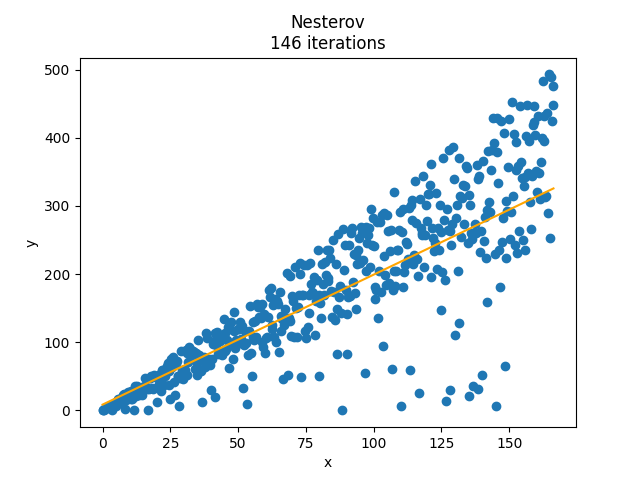
\includegraphics[scale=0.4]{nesterov_points.png}
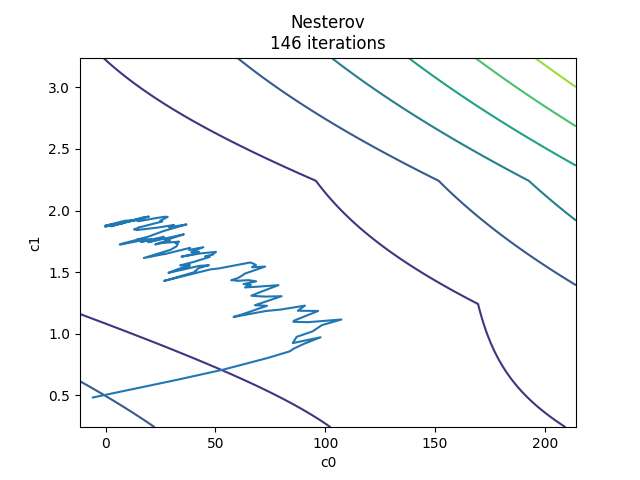
\includegraphics[scale=0.4]{nesterov_trace.png}

Здесь исходят из предположения, что основной вклад в вектор сдвига даёт первое слагаемое, а слагаемое с градиентом лишь “уточняет”. Логично поэтому уточняющий градиент расчитывать в окрестности новой точки, а не в текущей.

\subsection{Momentum}
Одна из проблем с SGD в том, что когда функция попадает в “овраг”, т.е. по одному из направлений имеем быстрый спуск, а по другому медленный, то SGD приводит к осциляции и крайне медленной сходимости к минимуму. \\
Для решения данной проблемы был предложен подход, который увеличивает шаг по направлению к минимуму, и уменьшает осциляцию. Это достигается за счёт того, что сдвиг параметров расчитывается как взвешенная сумма сдвига на предыдущем шаге и нового на основе градиента:

$$\Delta_{p + 1} = \gamma * \Delta_p + \eta *\Delta L(w_p)$$
$$w_{p + 1} = w_p-\Delta_{p+1}$$

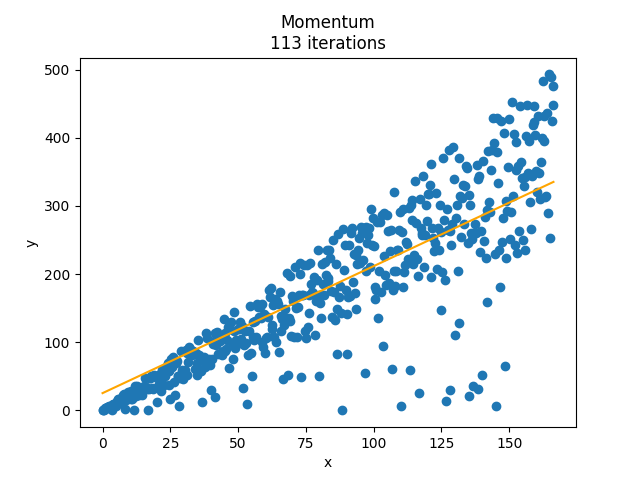
\includegraphics[scale=0.4]{momentum_points.png}
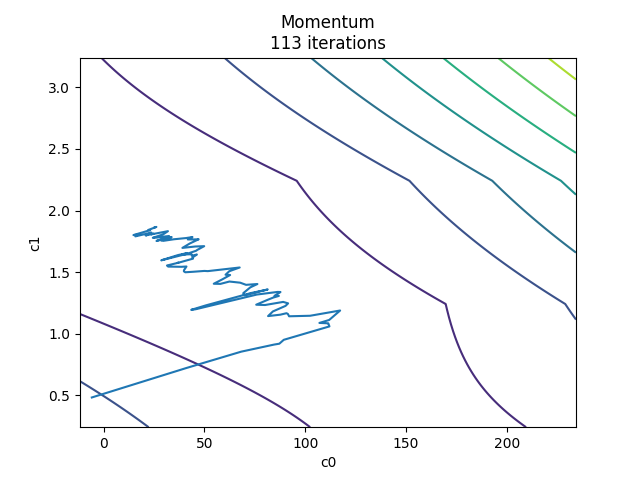
\includegraphics[scale=0.4]{momentum_trace.png}

\subsection{AdaGrad}
Вместо единого скаляра $\eta$ в качестве скорости обучения, на каждой итерации будем определять вектор $\eta_p=(\eta^{(1)}_p,…,\eta^{(d)}_p)$. \\
В данном случае $\eta$, которую мы использовали ранее будет просто начальной скоростью обучения. Для первой итерации мы положим $\eta^{(i)}_p=\eta,i=1,…,d$.

$$G^{(i)}_p = \sum_{j=1}^p{(g^{(i)}_j)^2},i=1,...,d$$
$$\eta^{(i)}_p = \frac{\eta}{\sqrt{G^{(i)}_p+\epsilon}}$$ \\

Изменение параметров осуществляем практически по той же формуле, что и раньше:
$$w_{p+1}=w_p−\eta_p * \Delta L(w_p)$$

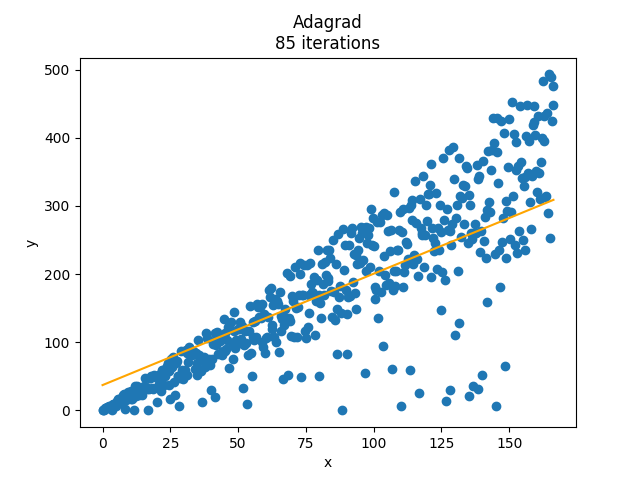
\includegraphics[scale=0.4]{adagrad_points.png}
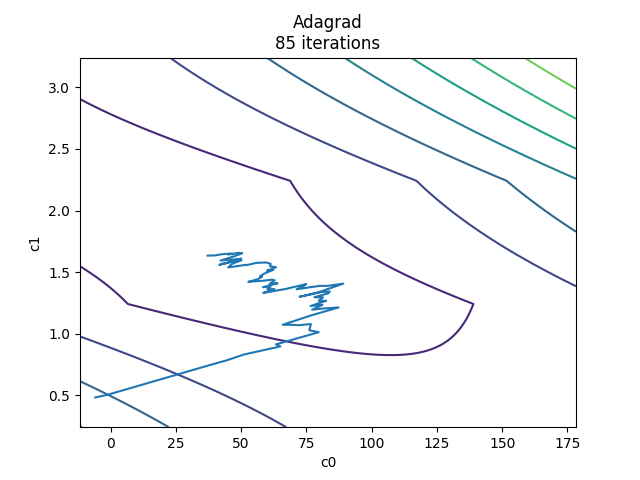
\includegraphics[scale=0.4]{adagrad_trace.png}

\subsection{RMSProp}
Основная проблема Adagrad заключается в том, что знаменатель в коэффициенте скорости обучения постоянно растёт, соответственно, через некоторое время для части параметров скорость обучения упадёт до нуля. \\
Так же Adagrad не избавляет нас от необходимости выбирать начальное значение $\eta$.

Предлагается следить за скользящим средним градиентов штрафной функции:

$$v_p=\beta * v_{p-1}+(1-\beta)⋅\Delta L(w_{p-1})^2$$

$$w_{p+1}=w_p - \eta*\frac{\Delta L(w_p)}{\sqrt{v_p}+\epsilon}$$

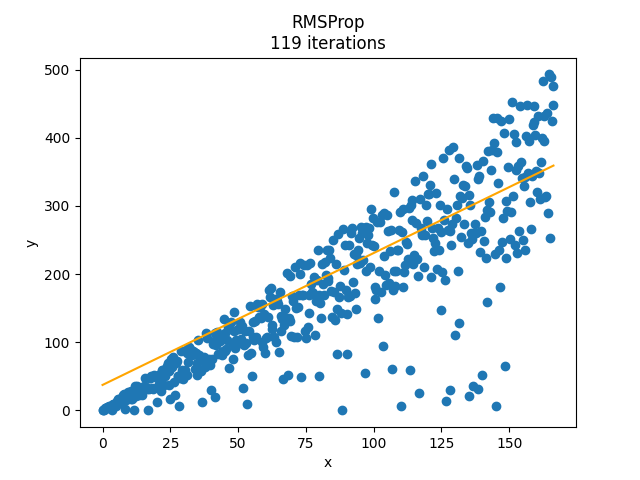
\includegraphics[scale=0.4]{rmsprop_points.png}
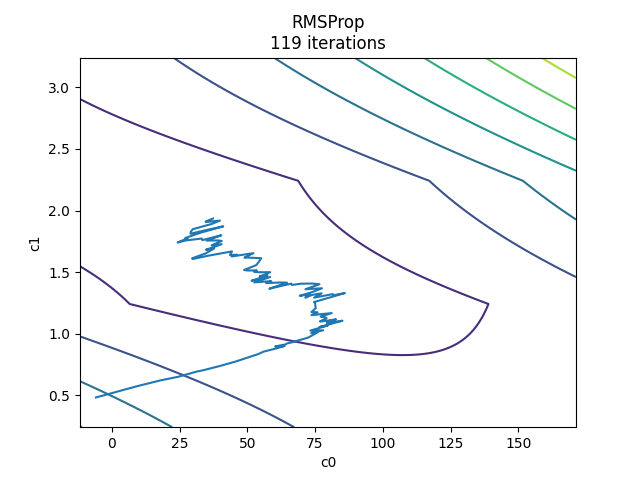
\includegraphics[scale=0.4]{rmsprop_trace.png}

\subsection{Adam}
Adam — один из самых эффективных алгоритмов оптимизации в обучении нейронных сетей. Он сочетает в себе идеи RMSProp и оптимизатора импульса. Вместо того чтобы адаптировать скорость обучения параметров на основе среднего первого момента (среднего значения), как в RMSProp, Adam также использует среднее значение вторых моментов градиентов. \\
В частности, алгоритм вычисляет экспоненциальное скользящее среднее градиента и квадратичный градиент, а параметры $\beta_1$ и $\beta_2$ управляют скоростью затухания этих скользящих средних.\\

Предлагается следить за скользящим средним градиентов и квадратов градиентов штрафной функции:

$$m_p=\beta_1 * m_{p-1}+(1-\beta_1)⋅\Delta L(w_{p-1})$$
$$v_p=\beta_2 * v_{p-1}+(1-\beta_2)⋅\Delta L(w_{p-1})^2$$

$$m'_p=\frac{m_{p}}{1 - \beta^p_1}$$
$$v'_p=\frac{v_{p}}{1 - \beta^p_2}$$

$$w_{p+1}=w_p - \eta*\frac{m'_p}{\sqrt{v'_p}+\epsilon}$$

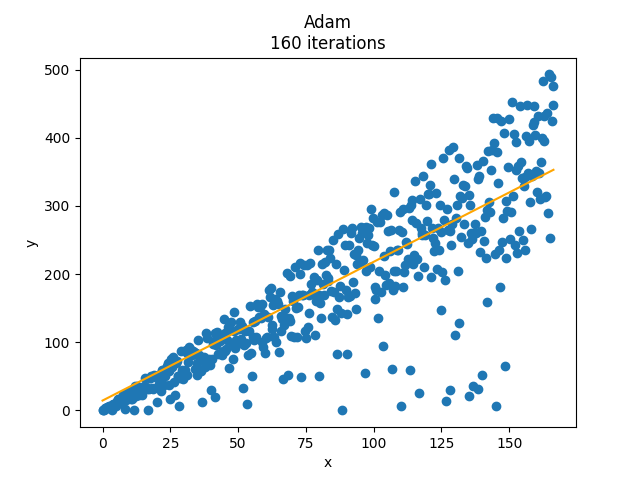
\includegraphics[scale=0.4]{adam_points.png}
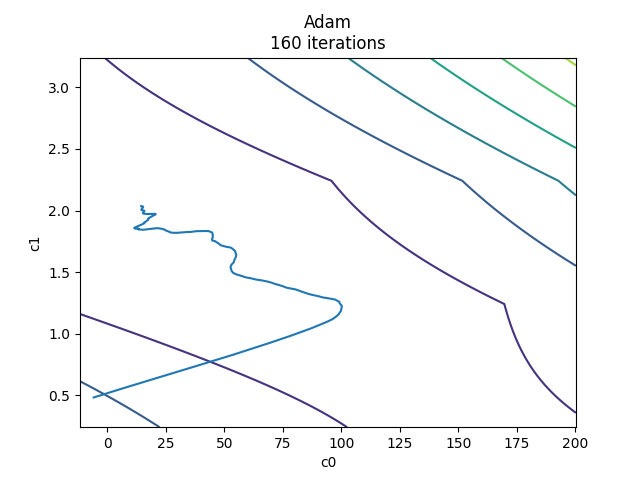
\includegraphics[scale=0.4]{adam_trace.png}

\section{Сравнение алгоритмов}

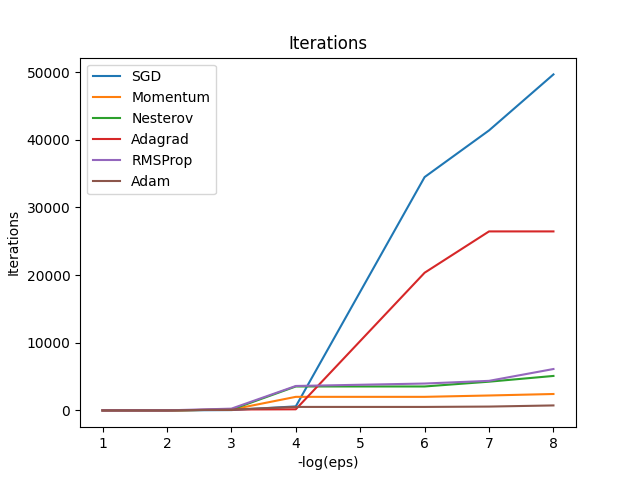
\includegraphics[scale=0.4]{iterations.png}
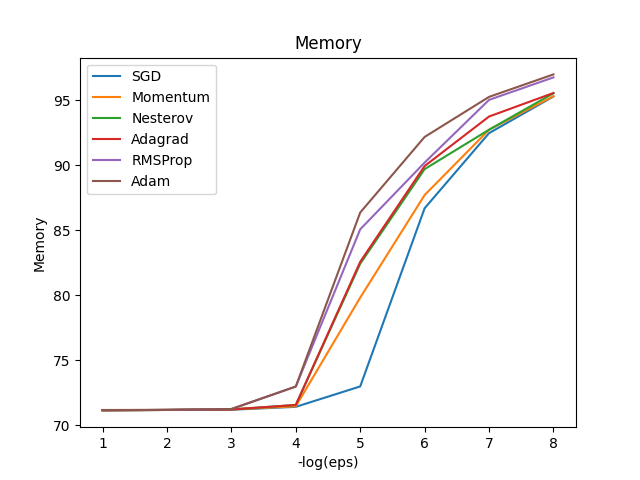
\includegraphics[scale=0.4]{memory.png}
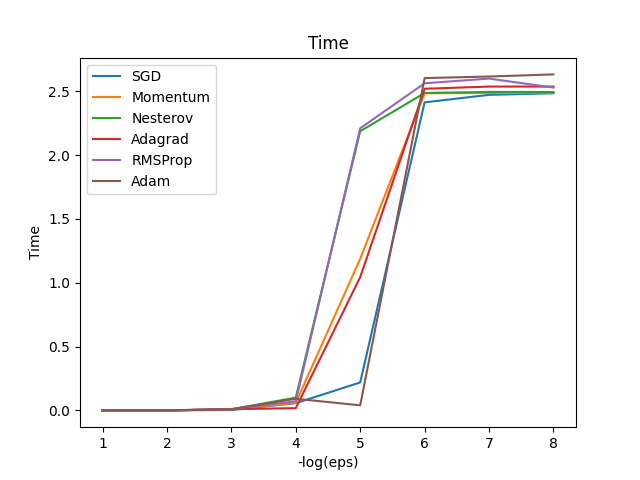
\includegraphics[scale=0.4]{time.png}

\end{document}
